\documentclass{article}
\usepackage{etex}
\usepackage[backend=biber]{biblatex}
\usepackage[]{hyperref}
\usepackage{graphicx}
\usepackage{booktabs}
\usepackage{siunitx}
\usepackage[]{amsmath}
\usepackage{gensymb}
\usepackage{mathtools}
\usepackage{fancyref}
\usepackage[table,xcdraw]{xcolor}
\usepackage{physics}
\usepackage{tikz}
\usepackage{pgfplots}

\addbibresource{/home/giorgio/Bibliography/bibliography.bib}
\hypersetup{
    colorlinks=true,
    linkcolor=blue,
    citecolor=blue,
    filecolor=magenta,      
    urlcolor=cyan,
    pdftitle={Esercitazioni Strutture per veicoli aerospaziali},
    bookmarks=true,
}
\usepgfplotslibrary{external}
\pgfplotsset{compat=1.5}
\tikzexternalize 
\author{De Trane Giorgio\\s275514}
\title{\textbf{Esercitazioni Strutture\\per Veicoli Spaziali}}

\begin{document}
    \setlength{\parindent}{0pt}
    \maketitle
    \begin{center}
        
\includegraphics[width=0.8\textwidth]{polito_logo.png}
        \linebreak
        \linebreak
        \textit{Anno accademico\\2020-2021}
    \end{center}
    \clearpage
    \tableofcontents
    \clearpage
    \section{Esercitazione 1\label{Esercitazione_1}}
    L'esercitazione é svolta utilizzando uno script in Fortran, messo a disposizione
    in un archivio denominato \textit{MUL2} \autocite{MUL2} e contenente anche un file di input ad hoc, in formato \textit{.dat},
    oltre a degli utili script di esempio per \textit{gnuplot} \autocite{gnuplot}, un libre software utilizzato poi per plottare tutti i grafici che seguono.
    \\
    \linebreak 
    In campo subsonico, con ripressurizzazione
    nulla e temperatura dell'aria di circa 23 °C, vale:
        \\ 
        \begin{equation}
            \phantomsection
            \label{tau_equation}
            \tau = 3.5 \cdot  10^{-3}\left ( \frac{V_c}{A_{eff}} \right )
        \end{equation}
        \\ 
        In campo sonico, con ripressurizzazione nulla e temperatura
        dell'aria di circa\linebreak 23 °C, vale:
        \\ 
        \begin{equation}
            \phantomsection
            \label{Omega_equation}
            \Omega \approx 0.025\left ( \frac{V_c}{A_{eff}} \right )\left [ (0.5283{\tilde{p}}^{o})^{\frac{1}{7}} - 1 \right ]
        \end{equation} 
        \\ 

    Sono state fatte diverse assunzioni per tutta 
    l'esercitazione:
    \begin{itemize}
        \item La depressurizzazione é:
            \begin{itemize}
                \item \textit{lenta} 
                        ($\displaystyle t > 10\, s$ \ ) 
                \item \textit{rapida} 
                        ($\displaystyle t < 10\, s$ \ )
                \item \textit{esplosiva} 
                        ($\displaystyle t < 500\, ms$ \ )
            \end{itemize}
        \item Il volume delle camere é \textit{costante}
        \item Il volume dell'atmosfera é supposto \textit{infinito}
        \item L'aria é trattata come \textit{gas ideale}
        \item Si utilizza un modello \textit{0D}, ossia con
              proprietá uniformi per tutta l'aria contenuta nel volume in analisi
        \item La quota rimane \textit{costante} durante la depressurizzazione
        \item L'effetto dell'umiditá relativa e dei calori latenti vengono trascurati
        \item Il modello utilizzato é di tipo quasi-stazionario, implementato attraverso un 
              \textit{algoritmo numerico}, il cui output fornisce 
              del feedback sugli input forniti e sulla supercriticitá (campo supersonico) o subcriticitá (campo subsonico)
              del fenomeno.

    \end{itemize}

    \begin{figure}[h!]
        \centering
        \phantomsection
        \label{fig:MUL2_stdout}
        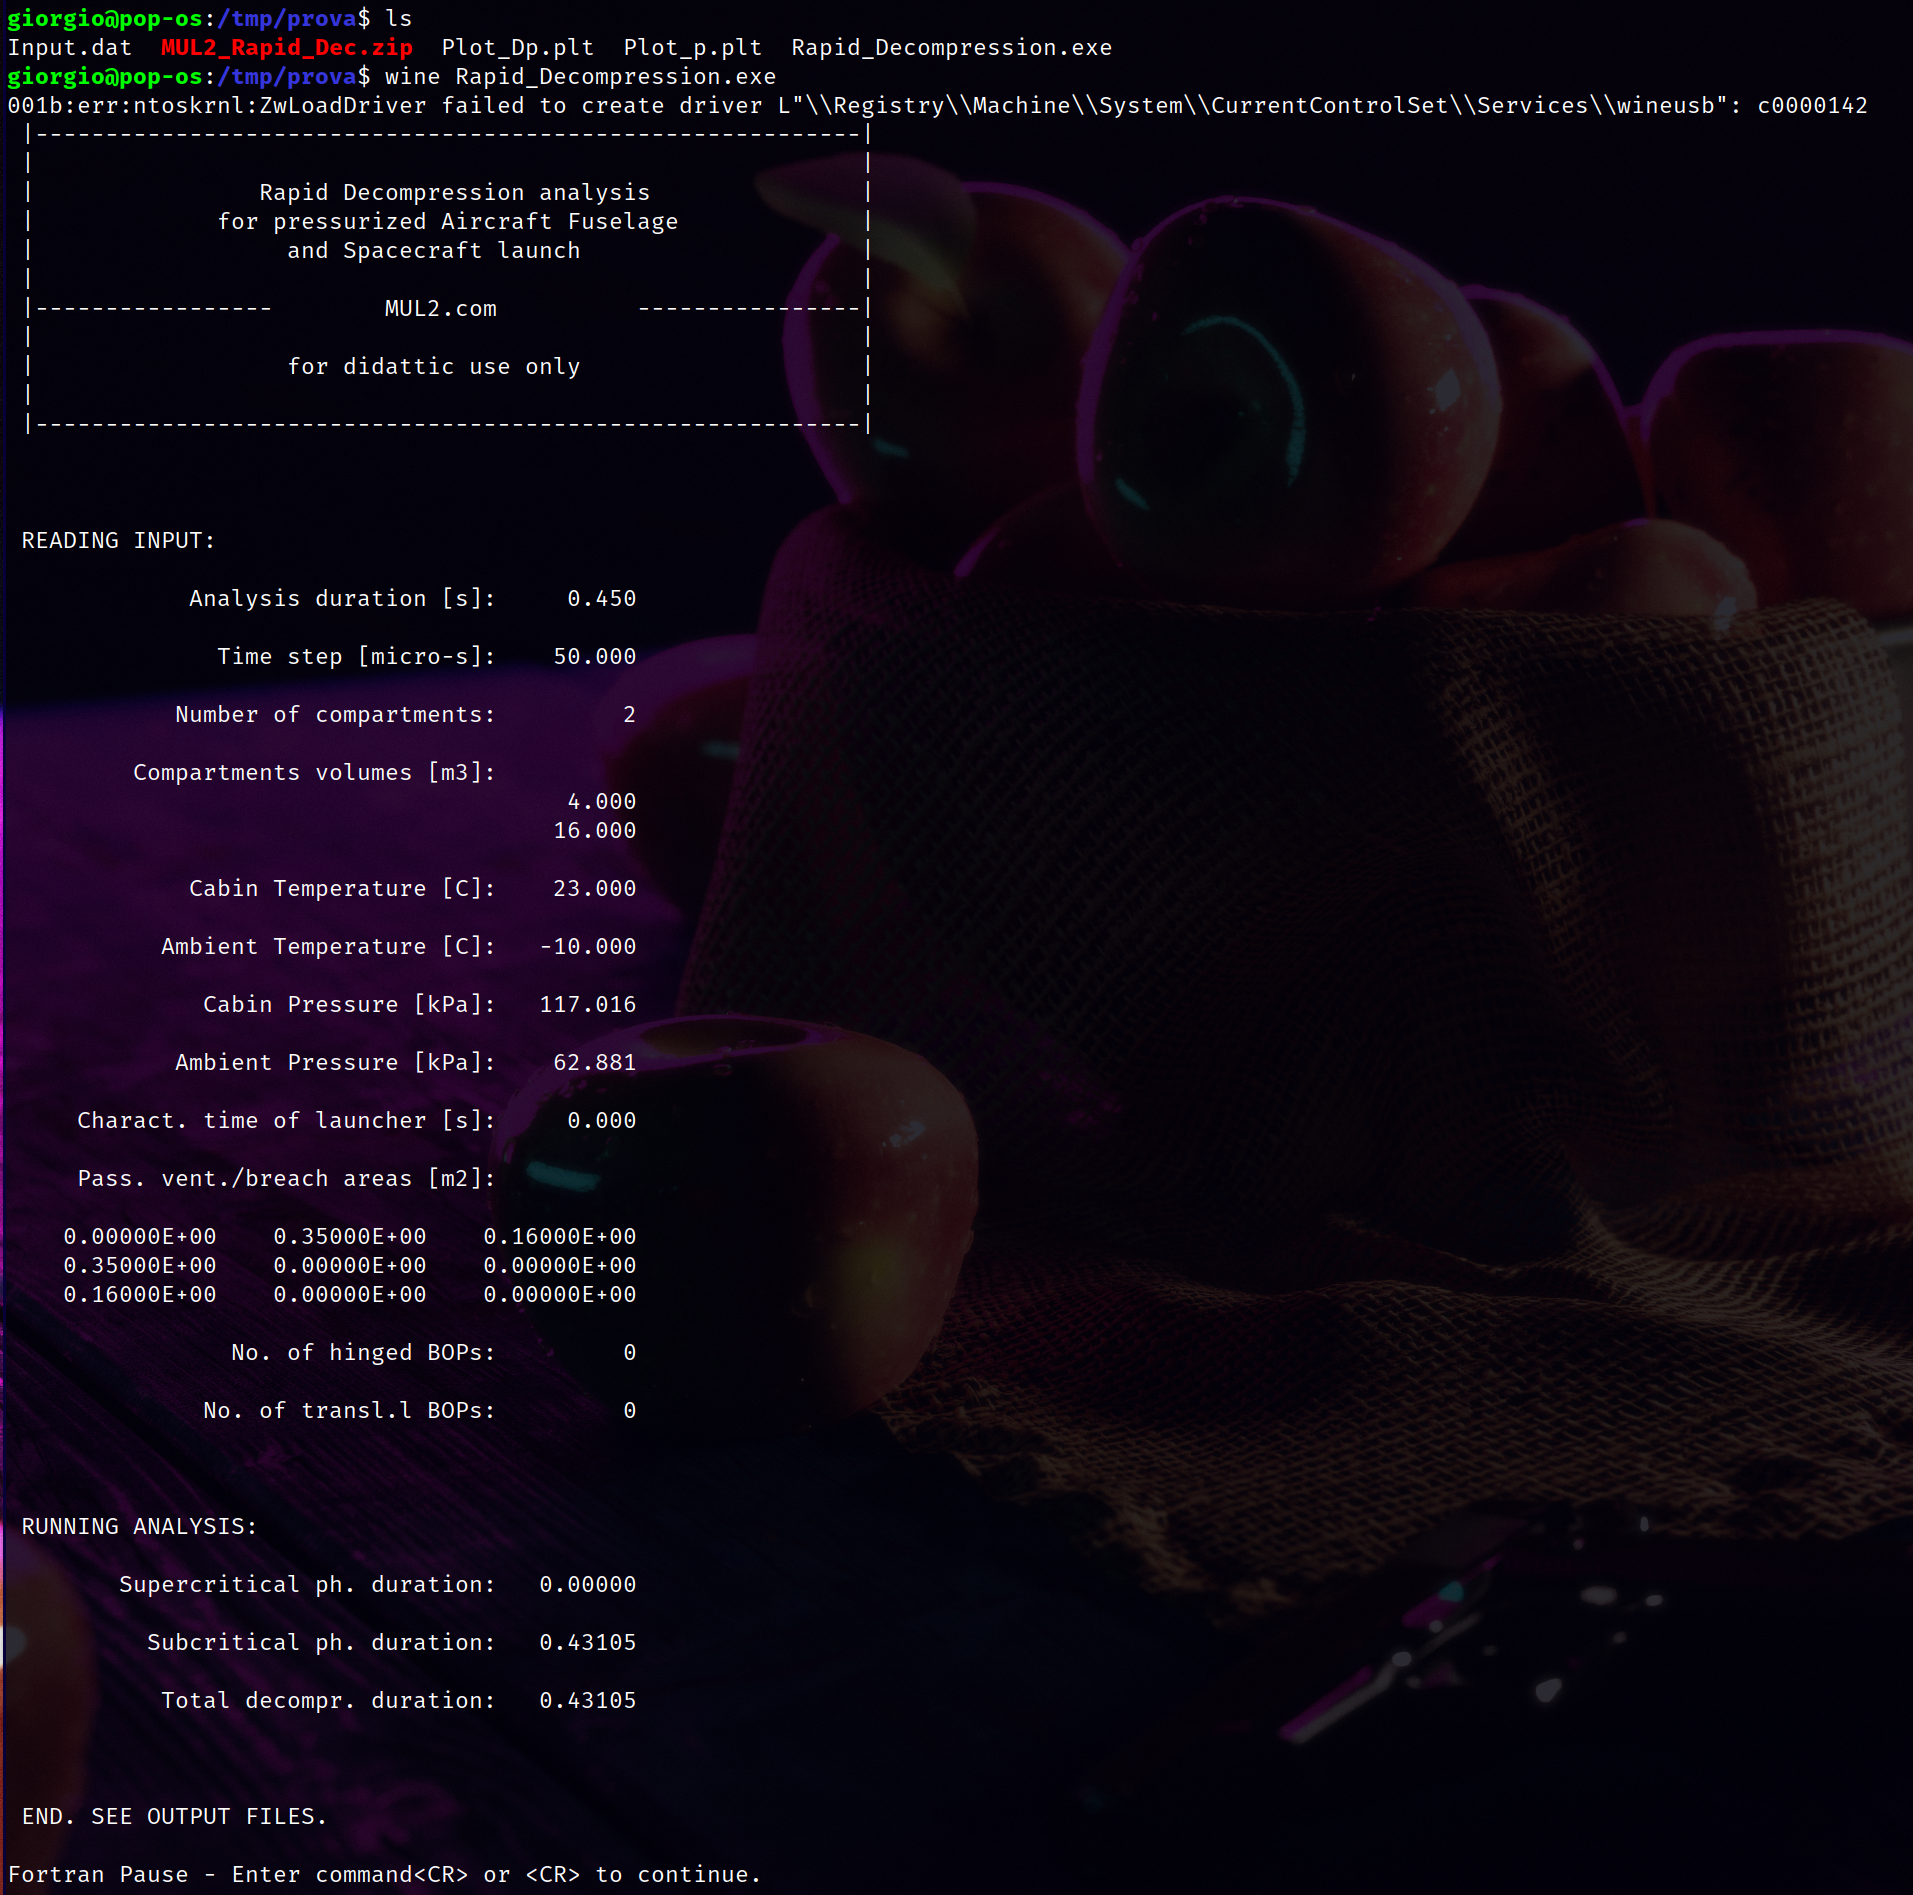
\includegraphics[width=\textwidth]{MUL2_feedback.png}\\
        \caption{stdout tipo}
    \end{figure}
    




    \clearpage

        \subsection{Esempio}
        Il caso esaminato é quello dell'Esempio 2, i cui dati sono quelli
        forniti di default nel file \textit{input.dat} .\\
        La configurazione in esame consiste in due camere comunicanti attraverso
        una ventilazione passiva, con un breach sull'ambiente esterno. 
        \begin{figure}[h!]
            \centering
            \phantomsection
            \label{fig:Esempio_2}
            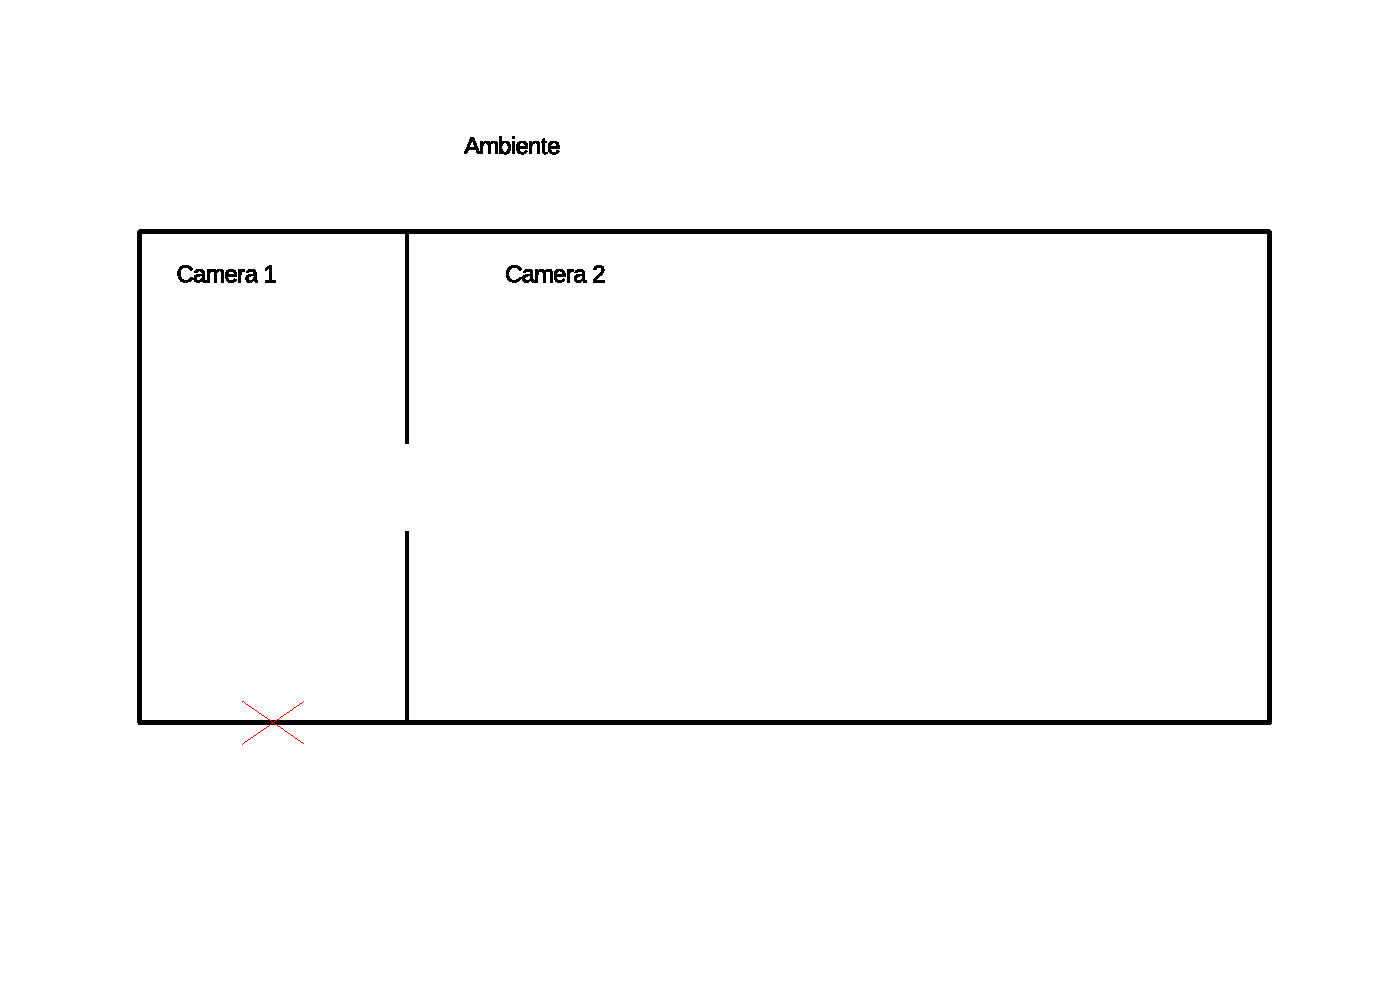
\includegraphics[width=0.7\textwidth]{ES1_Esempio2.eps}
            \caption{Esempio 2 (Disegnato con \textit{Inkscape} \autocite{Inkscape})}
        \end{figure}

        \subsubsection{DATI}
        \begin{itemize}
            \item $\displaystyle T_0 = -10\,°C;$ \
            \item $\displaystyle T_{c0} = 23\,°C;$ \
            \item $\displaystyle p_0 = 62.8812\,kPa;$ \
            \item $\displaystyle p_{c0} = 117.0162\,kPa;$ \
            \item $\displaystyle V_{C1} = 4\,m^3;$ \
            \item $\displaystyle V_{C2} = 16\,m^3;$ \
            \item $\displaystyle A_{1-0} = 0.2\,m^2;$ \
            \item $\displaystyle A_{1-2} = 0.5\,m^2;$ \
            \item $\displaystyle CD_{1-0} = 0.8;$ \
            \item $\displaystyle CD_{1-2} = 0.7;$ \
        \end{itemize}
        \clearpage

        \subsubsection{RISULTATI}
        
        Sono riportati i grafici ottenuti plottando i file di output
        generati dallo script.
        \begin{figure}[h!]
            \centering
            \phantomsection
            \label{fig:press_cam_ex}
            \includegraphics[width=0.6\textwidth, angle=-90]{MUL2/Esercitazione1/1A/p.eps}
            \caption{Pressioni di entrambe le camere nel tempo}
        \end{figure}

        \begin{figure}[h!]
            \centering
            \phantomsection
            \label{fig:grad_cam_ex}
            \includegraphics[width=0.6\textwidth, angle=-90]{MUL2/Esercitazione1/1A/Dp.eps}
            \caption{Gradiente di pressione tra le due camere}
        \end{figure}


        \clearpage
        \subsection{Esercizio 1\label{Es1}} 

        \begin{figure}[h!]
            \centering
            \phantomsection
            \label{fig:Esercizio_1}
            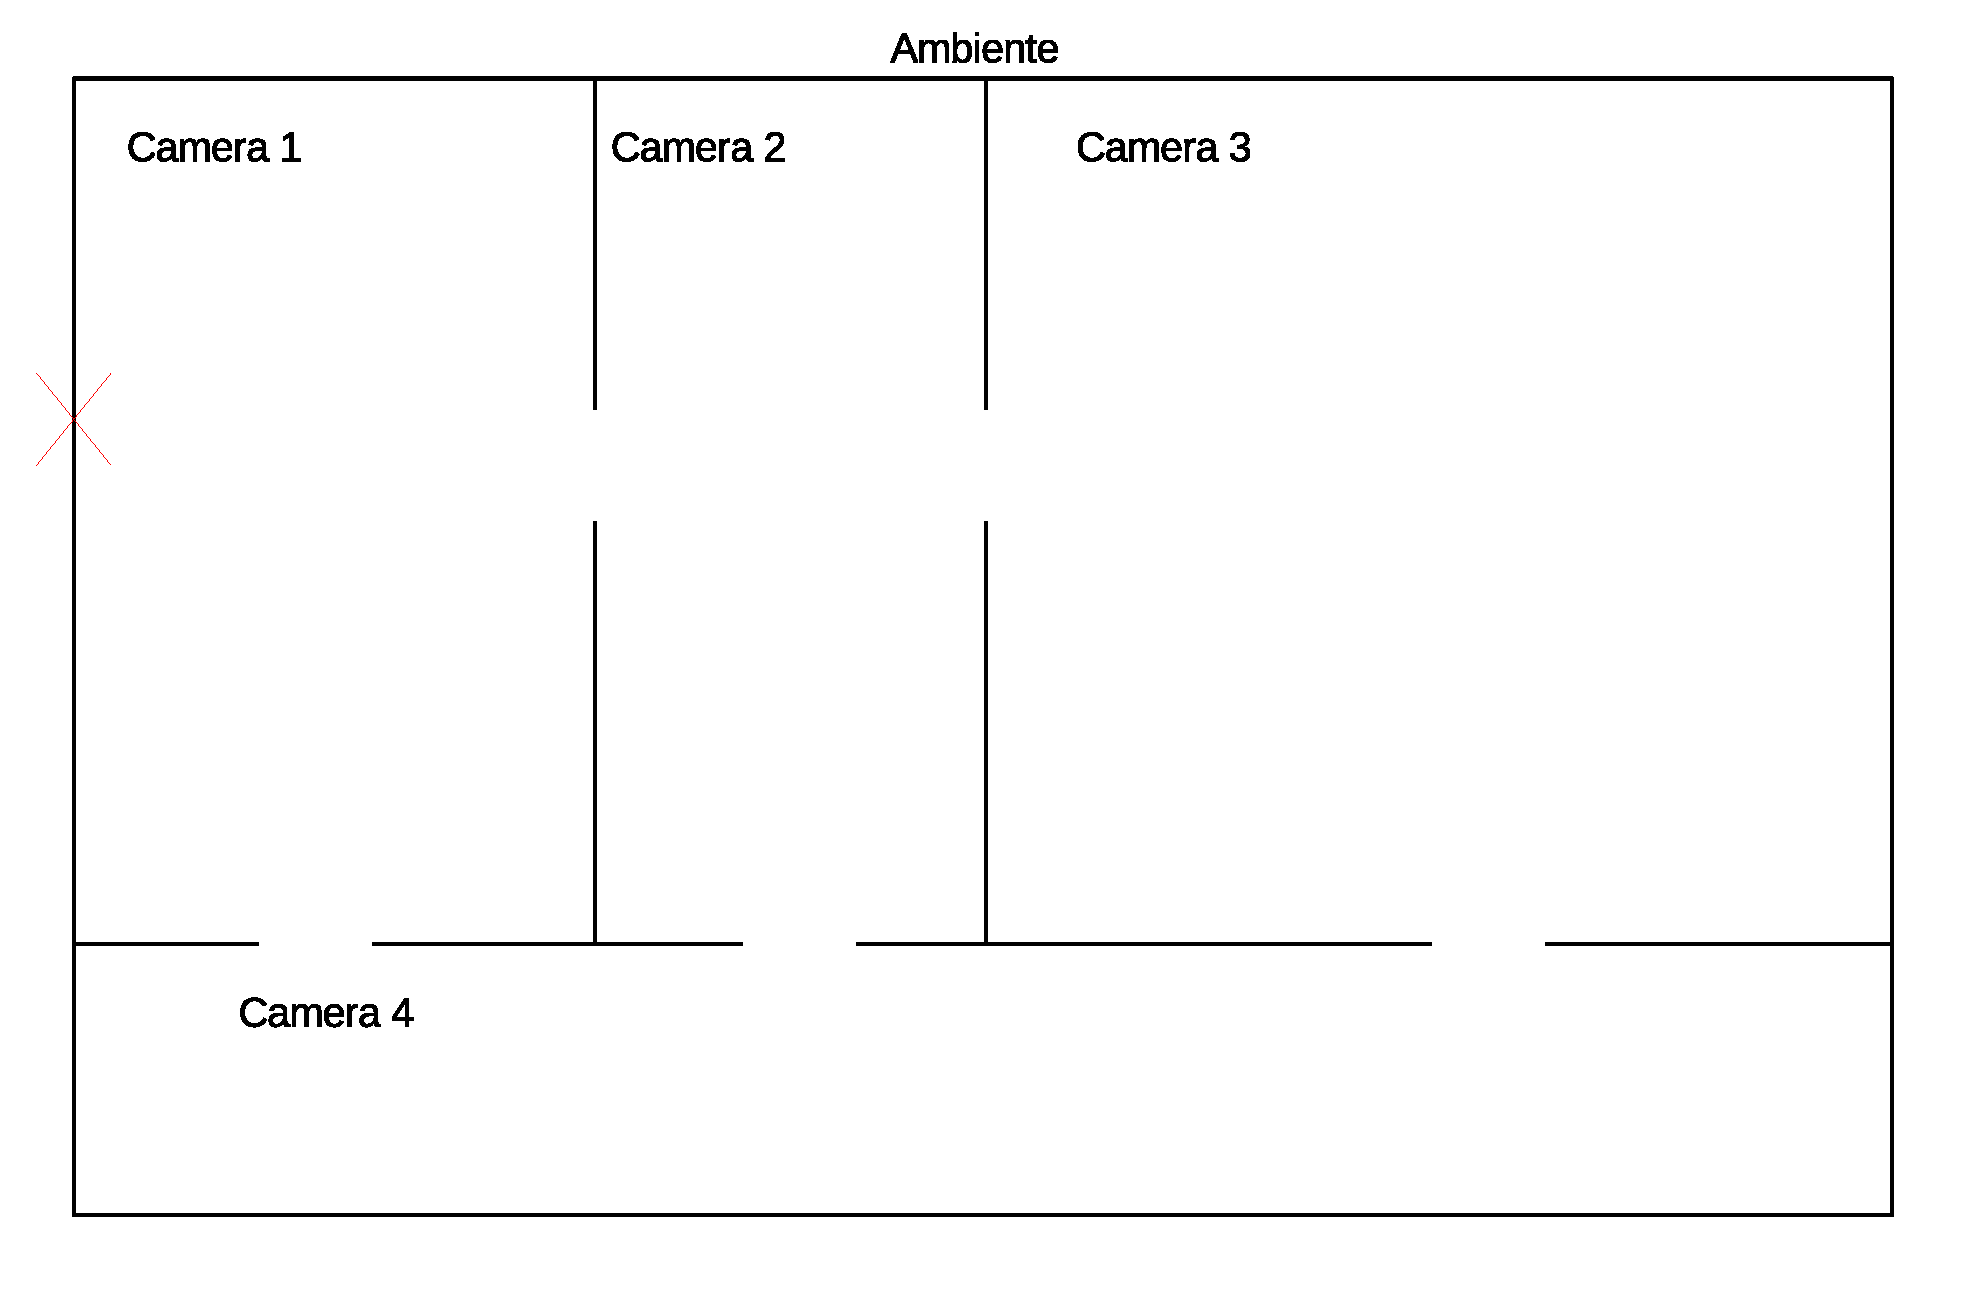
\includegraphics[width=0.5\textwidth]{ES1_Esercizio1.eps}
            \caption{Esercizio 1 (Disegnato con \textit{Inkscape} \autocite{Inkscape})}
        \end{figure}
        \subsubsection{DATI}
        \begin{itemize}
            \item $\displaystyle T_0 = -49.85\,°C;$ \
            \item $\displaystyle T_{c0} = 23\,°C;$ \
            \item $\displaystyle p_0 = 26.5\,kPa;$ \
            \item $\displaystyle p_{c0} = 89.876\,kPa;$ \
            \item $\displaystyle V_{C1} = 4\,m^3;$ \
            \item $\displaystyle V_{C2} = 3\,m^3;$ \
            \item $\displaystyle V_{C3} = 198\,m^3;$ \
            \item $\displaystyle V_{C4} = 67\,m^3;$ \
            \item $\displaystyle A_{1-0} = 1\,m^2;$ \
            \item $\displaystyle A_{1-2} = 0.6\,m^2;$ \
            \item $\displaystyle A_{2-3} = 0.6\,m^2;$ \
            \item $\displaystyle A_{1-4} = 0.8\,m^2;$ \
            \item $\displaystyle A_{3-4} = 0.8\,m^2;$ \
            \item $\displaystyle CD_{1-0} = 0.8;$ \
            \item $\displaystyle CD_{1-2} = [0, 0.5, 1];$ \
            \item $\displaystyle CD_{2-3} = 0.7;$ \
            \item $\displaystyle CD_{2-4} = 0.7;$ \
            \item $\displaystyle CD_{1-4} = 0.7;$ \
            \item $\displaystyle CD_{3-4} = 0.7;$ \
        \end{itemize}
        \clearpage
        \subsubsection{File di input}

        Il file di input viene modificato rispetto all'esempio, 
        inserendo ovviamente i dati forniti dal problema e rispettando la leggenda
        dello script.\\ 
        In particolare, la matrice delle aree effettive, ossia le singole aree fisiche che separano le camere, moltiplicate
        per i rispettivi coefficienti di efflusso, risulta: \\
        \begin{center}  
            \[
            \begin{pmatrix}
                0    & 0    & 0        & 0.56 & 0.8\\ 
                0    & 0    & 0.42     & 0.56 & 0\\ 
                0    & 0.42 & 0        & 0.56 & 0\\ 
                0.56 & 0.56 & 0.56     & 0    & 0\\
                0.8  & 0    & 0        & 0    & 0 
            \end{pmatrix}
            \]
            \\ 
            Per $\ CD_{1-2} = 0;$ \
            \\ 
            \[
            \begin{pmatrix}
                0    & 0.3  & 0        & 0.56 & 0.8\\ 
                0.3  & 0    & 0.42     & 0.56 & 0\\ 
                0    & 0.42 & 0        & 0.56 & 0\\ 
                0.56 & 0.56 & 0.56     & 0    & 0\\
                0.8  & 0    & 0        & 0    & 0 
            \end{pmatrix}
            \]
            \\ 
            Per $\ CD_{1-2} = 0.5;$ \
            \\ 
            \[
            \begin{pmatrix}
                0    & 0.6  & 0        & 0.56 & 0.8\\ 
                0.6  & 0    & 0.42     & 0.56 & 0\\ 
                0    & 0.42 & 0        & 0.56 & 0\\ 
                0.56 & 0.56 & 0.56     & 0    & 0\\
                0.8  & 0    & 0        & 0    & 0 
            \end{pmatrix}
            \]
            \\ 
            Per $\ CD_{1-2} = 1;$ \
        \end{center}    
        \clearpage

        \subsubsection{RISULTATI}
        Sono di seguito plottati gli andamenti delle pressioni e del 
        gradiente di pressione tra le camere 1 e 2, nel dominio del tempo. \\ 
        I plot sono ordinati a due a due per $\ CD_{1-2} = [0, 0.5, 1];$ \

        \begin{figure}[h!]
            \centering
            \phantomsection
            \label{fig:press_cam_0}
            \includegraphics[width=0.6\textwidth, angle=-90]{MUL2/Esercitazione1/1A/p.eps}
            \caption{Pressioni di entrambe le camere nel tempo}
        \end{figure}

        \begin{figure}[h!]
            \centering
            \phantomsection
            \label{fig:grad_cam_0}
            \includegraphics[width=0.6\textwidth, angle=-90]{MUL2/Esercitazione1/1A/Dp.eps}
            \caption{Gradiente di pressione tra le due camere}
        \end{figure}
        \clearpage
        
        \begin{figure}[h!]
            \centering
            \phantomsection
            \label{fig:press_cam_0.5}
            \includegraphics[width=0.6\textwidth, angle=-90]{MUL2/Esercitazione1/1B/p.eps}
            \caption{Pressioni di entrambe le camere nel tempo}
        \end{figure}

        \begin{figure}[h!]
            \centering
            \phantomsection
            \label{fig:grad_cam_0.5}
            \includegraphics[width=0.6\textwidth, angle=-90]{MUL2/Esercitazione1/1B/Dp.eps}
            \caption{Gradiente di pressione tra le due camere}
        \end{figure}
        \clearpage

        \begin{figure}[h!]
            \centering
            \phantomsection
            \label{fig:press_cam_1}
            \includegraphics[width=0.6\textwidth, angle=-90]{MUL2/Esercitazione1/1C/p.eps}
            \caption{Pressioni di entrambe le camere nel tempo}
        \end{figure}

        \begin{figure}[h!]
            \centering
            \phantomsection
            \label{fig:grad_cam_1}
            \includegraphics[width=0.6\textwidth, angle=-90]{MUL2/Esercitazione1/1C/Dp.eps}
            \caption{Gradiente di pressione tra le due camere}
        \end{figure}
        \clearpage

        \subsection{Esercizio 2\label{Es2}}

        Viene presa in analisi la depressurizzazione dell'\textit{UPM-Sat1} 
        \autocite{UPM_sat1}, in un tempo di 225 s. \\ 

        \begin{figure}[h!]
            \centering
            \phantomsection
            \label{fig:MUL2_stdout}
            \includegraphics[width=0.5\textwidth]{MUL2/Esercitazione1/2A/Esercizio_2.eps}
            \caption{\textit{UPM-Sat1} (Disegnato con \textit{Inkscape} \autocite{Inkscape})}
        \end{figure}

        L'analisi é svolta assumendo un \textit{coefficiente di efflusso} unitario,
        rispettando inoltre il modello fornito di depressurizzazione della camera esterna: la pressione
        inizialmente ha un determinato valore, che non puó piú essere considerato costante come nei casi precedenti, ma avrá un andamento 
        esponenziale del tipo: \\
        \begin{equation}
            \phantomsection
            \label{equation_press_exp}
            \frac{p_e}{p_i} = e^{-\left ({\frac{t}{t_p}}  \right )^2}
        \end{equation}

        Dove $t_p$ é un tempo caratteristico, pari a 0.75 s in questo caso.
        \\ 
        \linebreak
        Infatti, mentre il volume esterno era assunto infinito per l'Esercizio 1 (\ref{Es1}), va chiaramente considerato
        finito in questo caso, con la conseguenza che la pressione diminuisce.
        \\ 
        \linebreak
        Il volume dell'unica camera considerata é pari a $0.13 \ m^3$, mentre 
        l'area che la separa dall'esterno é presa in tre valori test differenti, ossia:
        \[24 \cdot \begin{bmatrix}
            10^{-5}\ m^2\ & 10^{-6}\ m^2\ & 10^{-7} \ m^2\
            \end{bmatrix}\]
        \clearpage

        \subsection{RISULTATI\label{Esercizio2_risultati}}
        Anche in questo caso, sempre tramite lo script in Fortran fornito a lezione, 
        vengono calcolate le pressioni nel tempo e il gradiente di pressione $\Delta p$ agente sulle pareti
        del satellite, plottando poi il tutto con \textit{gnuplot}.\\ 
        I plot sono ordinati a due a due, per ogni area considerata.
        
        \begin{figure}[h!]
            \centering
            \includegraphics[width=0.5\textwidth, angle=-90]{MUL2/Esercitazione1/2A/p.eps}
            \phantomsection
            \label{fig:press_10_5}
            \caption{Andamento delle pressioni} 
        \end{figure}

        \begin{figure}[h!]
            \centering
            \includegraphics[width=0.5\textwidth, angle=-90]{MUL2/Esercitazione1/2A/Dp.eps}
            \phantomsection
            \label{fig:grad_press_10_5}
            \caption{Andamento del gradiente di pressione}
        \end{figure}


        \clearpage

        \begin{figure}[h!]
            \centering
            \includegraphics[width=0.6\textwidth, angle=-90]{MUL2/Esercitazione1/2B/p.eps}
            \phantomsection
            \label{fig:press_10_6}
            \caption{Andamento delle pressioni} 
        \end{figure}

        \begin{figure}[h!]
            \centering
            \includegraphics[width=0.6\textwidth, angle=-90]{MUL2/Esercitazione1/2B/Dp.eps}
            \phantomsection
            \label{fig:grad_press_10_6}
            \caption{Andamento del gradiente di pressione}
        \end{figure}
        \clearpage

        \begin{figure}[h!]
            \centering
            \includegraphics[width=0.6\textwidth, angle=-90]{MUL2/Esercitazione1/2C/p.eps}
            \phantomsection
            \label{fig:press_10_7} 
            \caption{Andamento delle pressioni}
        \end{figure}
        
        \begin{figure}[h!] 
            \centering
            \includegraphics[width=0.6\textwidth, angle=-90]{MUL2/Esercitazione1/2C/Dp.eps}
            \phantomsection
            \label{fig:grad_press_10_7}
            \caption{Andamento del gradiente di pressione}
        \end{figure}

        \clearpage

        \subsection{Riflessioni}
        Dal primo Esercizio (\ref{Es1}), prendendo in analisi le prime due camere, si puó immediatamente notare come,
        a paritá di condizioni e di area comunicante tra i due volumi,
        il coefficiente di efflusso giochi un ruolo importante nel determinare l'andamento
        delle pressioni nelle due camere e, di conseguenza, il gradiente di pressione tra le due,
        a sua volta origine di carichi agenti sulla parete.\\ 
        Sono stati considerati tre casi, ossia il caso limite di efflusso nullo, quello di efflusso totale
        ed un caso intermedio.\\ 
        Nel caso di efflusso nullo (\ref{fig:press_cam_0}), la pressione decresce
        vertiginosamente entro pochi istanti nella prima stanza, con un picco piú elevato 
        rispetto agli altri casi, dopodiché resta costante, mentre nella seconda camera
        si ha una decrescita lineare piú lenta fino ad un picco piú basso che negli altri casi.\\ 
        Considerando un efflusso intermedio (\ref{fig:press_cam_0.5}), si puó giá 
        notare come la pressione nella prima camera decresca sí rapidamente, ma 
        fino ad un valore di picco meno elevato, per poi stabilizzarsi brevemente e riprendere con una decrescita molto lenta, 
        mentre nella seconda camera si ha una decrescita piú rapida del caso precedente e fino ad un valore di picco piú alto.
        \\ 
        Il trend é ancora piú evidente se si prende in considerazione un efflusso 
        totale (\ref{fig:press_cam_1}): la pressione della prima camera
        raggiunge un picco ancora piú basso e tende a decrescere un po' piú rapidamente
        dopo una breve stabilizzazione, ma comunque entro valori piú bassi dei casi precedenti, mentre 
        la seconda camera vede una decrescita di pressione ancora piú rapida
        e fino ad un picco piú alto.\linebreak
        \linebreak
        Quindi, dato che il gradiente é semplicemente calcolato come il valore assoluto
        della differenza tra i due profili di pressione, si nota immediatamente che, 
        all'aumentare del coefficiente di efflusso da 0 a 1, il suo valore
        massimo si minimizza e si ottiene anche una decrescita piú rapida.\\ 
        Da ció si deduce che, avere un efflusso troppo basso (o, peggio ancora, nullo)
        tra cabina e altri compartimenti in presenza di una breccia verso l'ambiente esterno, genera dei carichi di sollecitazione
        piú elevati, con possibili danni strutturali catastrofici.

        \clearpage

        
        Nel secondo Esercizio (\ref{Es2}), il coefficiente di efflusso viene assunto unitario
        ed il focus é sull'area che separa i due ambienti studiati.\\ 
        Nello specifico, vengono ancora una volta analizzate le pressioni tra le camere, 
        al fine di studiarne l'andamento del gradiente di pressione, 
        mettendo in risalto l'influenza che l'area di comunicazione puó avere.\\ 
        Il valore é ridotto, progressivamente nei tre casi,
        di un ordine di grandezza.\\ \linebreak
        Nel primo caso in questione, i due profili di pressione sono pressappoco identici (si ricorda che il modello utilizzato 
        é esponenziale (\ref{equation_press_exp})), per cui il gradiente ha un valore di picco molto basso (\ref{fig:grad_press_10_5}).\\ 
        Nel secondo caso l'area si riduce di un ordine di grandezza: i due profili
        di pressione cominciano a differenziarsi in maniera piú evidente per la scala studiata,
        ed il gradiente assume, come logico aspettarsi, un andamento analogo al precedente ma con un massimo significativamente
        piú elevato, di ben due ordini di grandezza per la precisione (\ref{fig:grad_press_10_6}).\\ 
        Nell'ultimo caso, l'area viene ulteriormente ridotta di un altro ordine di grandezza:
        stavolta gli andamenti delle pressioni si discostano sostanzialmente, con un decadimento
        molto piú rapido per la seconda camera.\\ 
        Di conseguenza, il gradiente risultante, pur mantenendo lo stesso tipo di 
        andamento, é cresciuto ulteriormente di un ordine di grandezza (\ref{fig:grad_press_10_7}).\\ 
        
    

        Si puó quindi intuire che, in una situazione di depressurizzazione, il ruolo dell'area di efflusso sia fondamentale
        nel tenere sotto controllo i carichi dovuti al gradiente di pressione: un'area troppo piccola
        potrebbe creare un gradiente eccessivamente alto e potenzialmente pericoloso per le
        strutture coinvolte.
        \clearpage
        \section{Esercitazione 2\label{Esercitazione_2}}

        Testo blablabla

        \begin{figure}[h!]
            \centering
            \phantomsection
            \label{fig:esercitazione2_drawing}
            
\includegraphics[width=0.8\textwidth]{MUL2/Esercitazione2/Esercitazione2.eps}
            \caption{Lanciatore (Disegnato con \textit{Inkscape} \autocite{Inkscape})}
        \end{figure}


        \begin{tikzpicture}[h!]
            \centering
            \begin{axis}[
                title=hi,
               
                colormap/cool,
            ]
            \addplot3[
                mesh,
                samples=50,
                domain=-8:8,
            ]
            {sin(deg(sqrt(x^2+y^2)))/sqrt(x^2+y^2)};
            \addlegendentry{$\frac{sin(r)}{r}$}
            \end{axis}
            \end{tikzpicture}

        \clearpage
        \printbibliography
\end{document}